\documentclass{article} % For LaTeX2e
\usepackage{nips13submit_e,times}
\usepackage{hyperref}
\usepackage{url}
\usepackage{graphicx}
\usepackage{epstopdf}
\usepackage{listings}
\lstset{language=Matlab}
\lstset{breaklines}
\lstset{extendedchars=false}
\usepackage{amsmath}
\usepackage{txfonts}
\usepackage{subfigure}
\usepackage{mathrsfs}



\title{Convolutional Neural Network and Convex optimization}


\author{
Si Chen  and   Yufei Wang\\
Department of Electrical and Computer Engineering\\
University of California San Diego\\
\texttt{\{sic046, yuw176\}@ucsd.edu}          \\
}

% The \author macro works with any number of authors. There are two commands
% used to separate the names and addresses of multiple authors: \And and \AND.
%
% Using \And between authors leaves it to \LaTeX{} to determine where to break
% the lines. Using \AND forces a linebreak at that point. So, if \LaTeX{}
% puts 3 of 4 authors names on the first line, and the last on the second
% line, try using \AND instead of \And before the third author name.

\newcommand{\fix}{\marginpar{FIX}}
\newcommand{\new}{\marginpar{NEW}}

\nipsfinalcopy % Uncomment for camera-ready version

\begin{document}


\maketitle
\begin{abstract}
%We model the relationship between sentences and their punctuation labels using conditional random fields. Some feature functions are hand-designed and others are generated by templates. We train the same model by stochastic gradient ascent, Collins Perceptron and contrastive divergence respectively and compare their performance. On the provided dataset, we achieve word-level accuracy of 94.56\%. At last, we propose a heuristic that can deal with cost-sensitive tasks.   
Latent Dirichlet allocation(LDA) is a generative topic model to find latent topics in a text corpus. It can be trained via collapsed Gibbs sampling. In this project, we train LDA models on two datasets, Classic400 and BBCSport dataset. We discuss possible ways to evaluate goodness-of-fit and to detect overfitting problem of LDA model, and we use these criteria to choose proper hyperparameters, observe convergence, and evaluate the models, the criteria we use include perplexity, VI-distance, visualization of clustering results, and highest-probability words. 

\end{abstract}
\section{Introduction}

Deep learning


Convex optimization


SVM-loss



%Latent Dirichlet allocation introduced by \cite{blei} is a generative probabilistic model for collection of discrete data, such as text corpora.It assumes each word is a mixture over an underlying set of topics, and each topic is a mixture over a set of topic probabilities. Evaluating the models is a tough issue. There are several types of methods that people use: The models can be applied to some tasks such as document classification, where the performance can be easily evaluated; Several methods estimate the likelihood of held-out documents; Subjective judgement can be made by examine word and document similarities. In this project, we learn the models of two datasets, Classic400 and BBCSport dataset, by collapsed Gibbs sampling, and use several methods to evaluate the models, including perplexity, VI-distance, visualizing result and highest-probability words.
\par
%This report is organized as follows. Section 2 gives a brief overview of LDA model and training process, and introduces several methods to evaluate goodness-of-fit and check overfitting. We describe some implementation details in Section 3. In Section 4, we describe the design of our experiments. Section 5 shows the experiment results with discussions. Finally, we draw some conclusions in Section 6.

\section{Sub-model Convolutional Network}
\subsection{Theoretical basis: Convolutional neural network}
Convolutional neural networks(CNN) are a special kind of deep neural networks. It exploits local correlation by enforcing a local connectivity pattern between neurons of adjacent layers. For a certain hidden layer $m$, the hidden units in it are connected to a local subset of units in the $(m-1)$th layer. Additionally, each sparse filter $h_{i}$ is replicated across the entire visual field. The replicated units share the same parametrization, i.e. the same weight vector and same bias. The layer is called feature map. 
\par
Mathematically, a feature map $h^{k}$ is obtained by convolving the input with a linear filter, adding a bias term and then applying a non-linear function, it can be shown as follow:
\begin{equation}
h^{k}_{ij}=\textup{f}((W^{k}*x)_{ij}+b_{k})
\end{equation}
where $W^{k}$ and $b_{k}$ are weight and bias of $k$th feature map, and $\textup{f}(\cdot)$ is the nolinearity. In our experiments, Rectified Linear Units(ReLU) nonlinearity is used, which has been shown to be more efficient than conventional function $\textup{tanh}(\cdot)$.\cite{imagenet} ReLU nonlinearity is as follow:
\begin{equation}
f(x)=\textup{max}(0,x)
\end{equation}
\par
Another important type of layers is pooling. It is a form of non-linear down-sampling. There are several types of pooling, two common types of which are max-pooling and average-pooling. They partition the input image into a set of non-overlapping or overlapping rectangles and outputs the maximum/average value for each such sub-region. By pooling, the model can reduce the computational complexity for upper layers, and can provide a form of translation invariance. 
\par
Typically, the last layer of a CNN is a logistic regression layer. Each unit of the output reflects a class membership probability:
\begin{equation}
P(Y=i|x,W,b)=softmax_{i}(Wx+b)=\frac{e^{W_{i}x+b_{i}}}{\sum _{j}e^{W_{j}x+b_{j}}} 
\end{equation}
\par
The parameters of the network are trained using back propagation\cite{backprop}. The loss function used for training is the negative-log likelihood of the training dataset $D$ under the model:
\begin{equation}
L = \sum_{i=0}^{|D|}\textup{log}(P(Y=y^{(i)}|x^{(i)},W,b))
\end{equation}
\par
Finally, the prediction of the model is done by taking the argmax of the vector of $P(Y=i|x,W,b)$:
\begin{equation}
y_{pred}=\textup{argmax}_{i}P(Y=i|x,W,b)
\end{equation}

\subsection{Overall architecture}
The overall architecture of our CNN is shown in Figure~\ref{fig1}. There are three convolutional layers and pooling layers alternatively. Overlapping pooling is performed. Each pooling layer consists of a grid of pooling units spaced $s=2$ pixels apart, each summarizing a neighborhood of size $3\times3$ centered at the location of the pooling unit. The output of the network is a vector of class membership probability with 10 units, corresponding to 10 classes in our CIFAR-10 dataset\footnote{http://www.cs.toronto.edu/~kriz/cifar.html}.

\begin{figure}
\centering
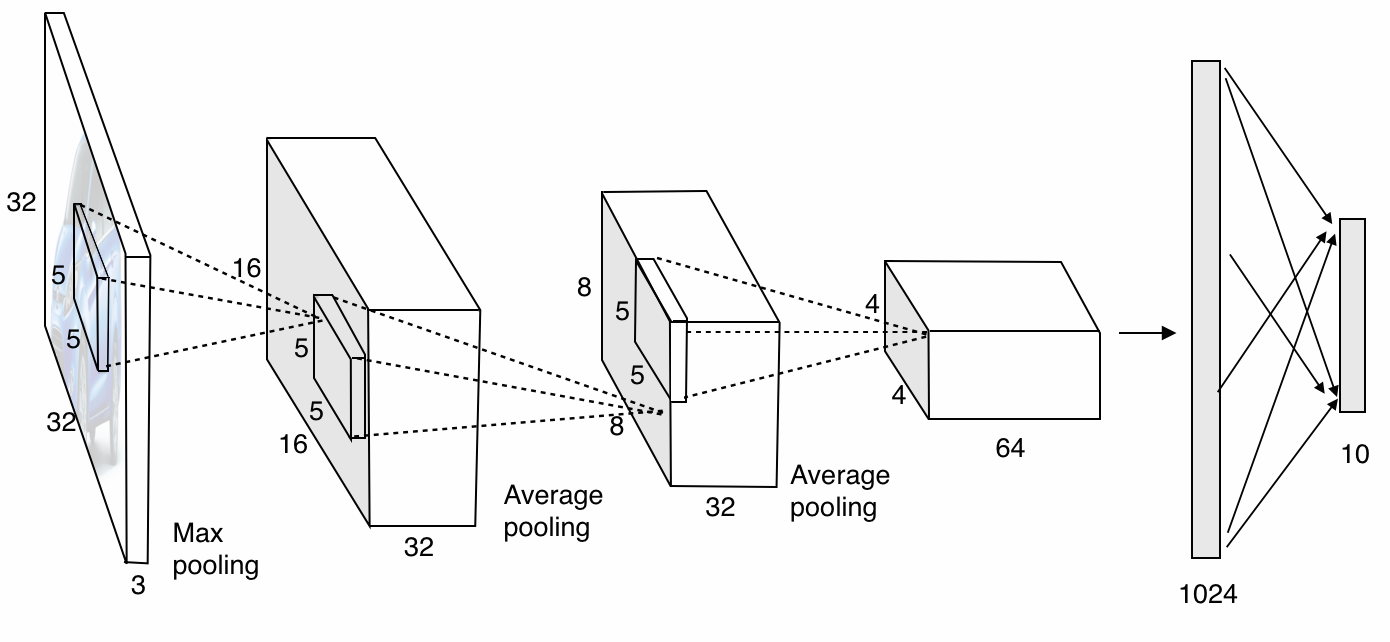
\includegraphics[width=1\textwidth]{architecture}
\caption{The architecture of our CNN.}
\label{fig1}
\end{figure}
\subsection{Dropout and sub-model combination}
Dropout is a recently-introduced technique to reduce overfitting \cite{imagenet}. It consists of setting to zero the output of each hidden neuron with probability of 0.5 in training procedure.  So every time a training example is presented, the neural network samples a different architecture, which we denote here as a sub-model $m_{k}$. All these sub-models share weights. At test time, we use all neurons but multiply their outputs by 0.5, which is an approximation to taking the geometric mean of the predictive distributions $P_{m_{k}}=\left [ P_{m_{k}}(Y=1),P_{m_{k}}(Y=2),...,P_{m_{k}}(Y=d) \right ]^{t}$ produced by the sub-models (where $d$ is the number of classes):

\begin{equation}
\begin{split}
(P_{m_{1}}(Y=i)\cdot P_{m_{2}}(Y=i)\cdot\cdot \cdot \cdot P_{m_{n}}(Y=i))^{\frac{1}{n}}&=\frac{e^{(b_{i}+W_{i}\frac{1}{n}\sum_{k=1}^{n}h_{m_{k}})}}{(\sum_{j=1}^{d}e^{(nb_{j}+W_{j}\sum_{k=1}^{n}h_{m_{k}})})^{\frac{1}{n}}}
 \\
           &= \frac{e^{(b_{i}+W_{i}\cdot h_{comb})}}{(\sum_{j=1}^{d}e^{(nb_{j}+W_{j}\sum_{k=1}^{n}h_{m_{k}})})^{\frac{1}{n}}}
\end{split}
\end{equation}
\begin{equation}
P_{comb}(Y=i)=\frac{e^{b_{i}+W_{i}\cdot h_{comb}}}{\sum_{j=1}^{d}e^{b_{j}+W_{j}\cdot h_{comb}}}
\end{equation}

where $h_{m_{k}}$ is the neurons of the penultimate layer of sub-model $m_{k}$, and $h_{comb}$ is the that of the combined model by using all the neurons but multiply them by 0.5. $P_{comb}(\cdot)$ is the class membership probabilities of the combined model. 
\par
Apparently, the predictive distribution of the combined model is only a biased approximation of taking the mean of the predictive distribution of all sub-models.
\par
In our experiments, the architecture is shown in Figure~\ref{fig1}, dropout is performed in the output of penultimate layer, and $d=10$ is the number of classes of our dataset.
\par
Here, we want to explore a better option of combining the sub-models. Rather than giving an approximation, we want to actually taking the linear combination of the predictive distribution of $n$ sub-models:
\begin{equation}
P_{l.comb}(Y=i) = \sum_{k=1}^{n}l_{k}\times P_{m_{k}}(Y=i)
\end{equation}
where $l_{k}$ is the weight of the distribution of $k$th model. The best weight $l=\left[ l_{1},l_{2}, ..., l_{n}\right]^{t}$ can be obtained solving following optimization problem:
\par
\setlength{\parindent}{3em}
minimize $\sum_{i=1}^{N}\left \| P_{i}\cdot l-y_{i} \right \|_{2}^{2}$,
\par
\setlength{\parindent}{3em}
subject to $l\succeq 0$.
\setlength{\parindent}{0pt}
\par
with the variable $l$, where $N$ is the number of all the training examples, $y_{i}$ is the $10 \times 1$ binary column vector indicating the true label of $i$th data point, and $P_{i} =\left [ P_{m_{1}},P_{m_{2}},...,P_{m_{n}} \right ] $ is a $10 \times n$ matrix. By minimizing the sum of squared l2 norm of difference between predicted distribution and true label, we find the non-negative weight vector $l$.
\par
The objective function can be simplified as following:
\begin{equation}
\begin{split}
\sum_{i=1}^{N}\left \| P_{i}\cdot l-y_{i} \right \|_{2}^{2} &=\sum_{i=1}^{N}(P_{i}\cdot l-y_{i})^{t}(P_{i}\cdot l-y_{i})
 \\
&=(P\cdot l-y)^{t}(P\cdot l-y)
 \\
&=l^{t}P^{t}Pl-2y^{t}Pl+y^{t}y
\end{split}
\end{equation}
where $y = \left[ y_{1}^{t}, y_{2}^{t},...y_{N}^{t}\right]^{t}$ is the concatenation of label indicator vectors of all data points, which is a $10N\times 1$ vector. $P = \left[ P_{1}^{t},P_{2}^{t},..., P_{n}^{t}\right]^{t}$ is the concatenation of probability distributions of all data points, which is a $10N \times n$  matrix. Then the optimization problem can be written as follow:
\par
\setlength{\parindent}{3em}
minimize $l^{t}P^{t}Pl-2y^{t}Pl+y^{t}y$,
\par
\setlength{\parindent}{3em}
subject to $l\succeq 0$.
\setlength{\parindent}{0pt}
\par
with the variable $l$. This is a Quadratic Optimization Problem (QP), apparently a convex optimization problem, and is easy to solve.



\subsection{Sub-model combination in non-dropout CNN}
Now let's move back to CNN without dropout training. The same idea of sub-model combination can also be utilized to improve the performance of CNN when the network is trained without dropout. 
\par
The sub-models can be obtained by similar fashion with the dropout sub-models: given the already trained CNN model without dropout, randomly set penultimate units to zero with probability of 50\%, and multiply the remaining units by 2:
\begin{equation}
\textup{Pr}(h_{m_{i}}^{j}=2h_{orig}^{j})=\textup{Pr}(h_{m_{i}}^{j}=0)=\frac{1}{2}.
\end{equation}
where  $h_{m_{i}}$ is the 1024 penultimate-layer unit vector of the sub-model $m_{i}$, $h_{orig}$ is the 1024-unit vector of the trained CNN model, and $h_{(\cdot)}^{j}$ is the $j$th element of the vector. 
\par
Then, we can obtain the predictive distribution of each sub-model $P_{m_{k}}$, and the new model takes linear combination of the predictive distribution of $n$ sub-models, which is the same as the dropout condition:
\begin{equation}
P_{l.comb}(Y=i) = \sum_{k=1}^{n}l_{k}\times P_{m_{k}}(Y=i)
\end{equation}
\par
Therefore, the optimization problem is very similar with dropout condition, and the only difference is the multiplication by 2 when obtaining the penultimate layer of sub-models.

\section{Multiclass}


\section{Experiments}
\subsection{Sub-model convolutional network}
We use Theano\cite{theano} to train and test the CNN model, and cvx toolbox\footnote{http://cvxr.com} in matlab to solve the convex optimization problem finding best weights. The training and test data are CIFAR-10 dataset.
\par
We separately train the model with and without dropout, and the the result on the test set is shown in \ref{table1}. Accuracy of dropout network is about 2\% higher than nondropout network, which shows the advantage of dropout method.
\par
Then, we randomly extract 4800 sub-models from dropout/non-dropout network respectively, find the optimal weight $l$ by solving the convex optimization problem using different number of sub-models. The plot of the accuracy on test set versus number of sub-models is shown in Figure~\ref{accuracies}. The dotted line in both figures are the accuracy of the original model, which is the approximation of geometric mean of all possible sub-models.
\par 
Clearly, the accuracy tend to increase with the number of sub-models used. This is intuitive: the sub-models are chosen randomly, the more sub-models we use, the more probable we have useful sub-models and better combinations. As is shown in Figure~\ref{accuracies}(a), for the model trained by dropout, the improvement is limited: approximately 0.2\% improvement is achieved. However, for model trained without dropout, the improvement by weighted combination of sub-models is much more significant: the accuracy of original model is 79.52\%, and the weighed combination of sub-models is always better than the original model, even when there are only 100 sub-models. The improvement is up to ???? when the number of sub-models reaches to ???.
\par
\begin{figure}
\centering 
\subfigure[Accuracy-number of sub-models for dropout network]{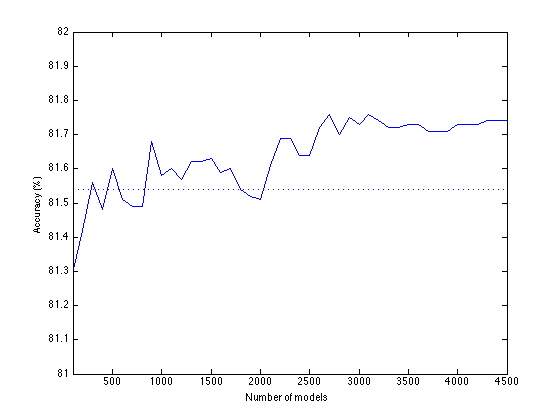
\includegraphics[width=0.8\textwidth]{dropout.png}} 
\subfigure[Accuracy-number of sub-models for nondropout network]{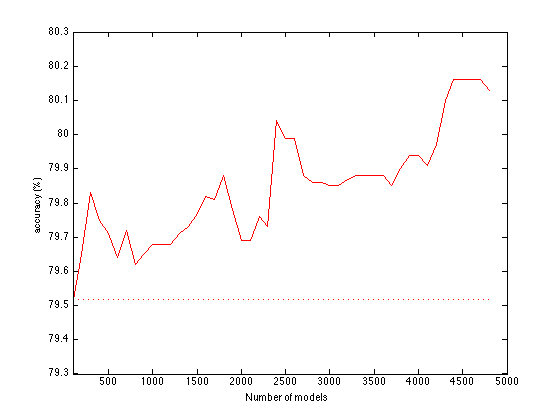
\includegraphics[width=0.8\textwidth]{nodropout.png}} 
\caption{ Accuracy-number of sub-models.}
\label{accuracies} 
\end{figure}

\subsection{The role of dropout}
The reason of the lower improvement for dropout network is explained in this section. Dropout training trains different sub-model at a time, but the weights are shared by all the sub-models. This procedure forces the network to learn more robust features that are useful for many different random sub-models, and after training, the sub-models in the dropout network can give similar results for all the data. This is the eventual goal of the dropout training. In other words, the sub-models in the dropout network are similar to each other, therefore whatever combination of them would not achieve much improvement. On the other hand, the network trained without dropout doesn't have the invariant property, thus the sub-models are quite different to each other, leading to greater improvement by combining them.
\par
Figure~\ref{hist} illustrates this effect of dropout training clearly. accuracies achieved by 4800 sub-models for nondropout/ dropout network are shown in the two histograms. Clearly, the sub-models of dropout network are much more concentrated than those of the nondropout network. This shows the larger variance of the sub-models in nondropout network.
\begin{figure}
\centering 
\subfigure[Histogram of accuracies of sub-models of dropout network]{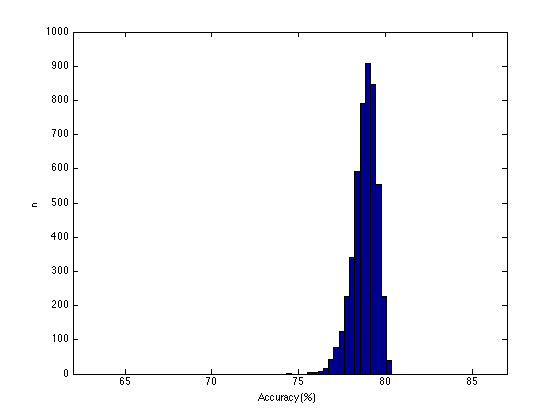
\includegraphics[width=0.8\textwidth]{dropout_hist.png}} 
\subfigure[Histogram of accuracies of sub-models of nondropout network]{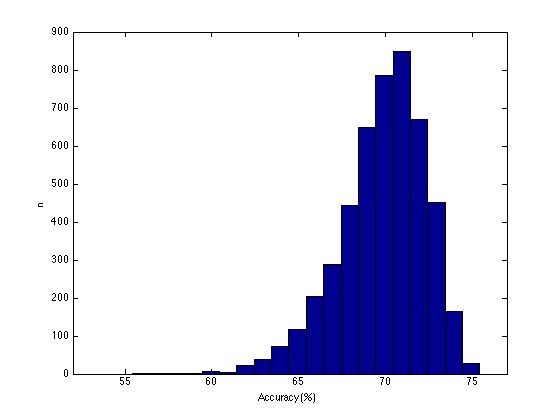
\includegraphics[width=0.8\textwidth]{nodropout_hist.png}} 
\caption{ Histograms of sub-models.}
\label{hist} 
\end{figure}

\begin{table}
\centering 
    \begin{tabular}{l|l}
    \hline
    Network     & Accuracy on test set (\%) \\ \hline
    Dropout     & 81.540                 \\ \hline
    Non-dropout & 79.517                 \\ \hline
    \end{tabular}
     \caption{Accuracy of networks}   
     \label{table1}
\end{table}

\section{Conclusion}

\bibliographystyle{splncs}
\bibliography{ECE273}
\end{document}